\chapter{Local Correlation: Excited State}

The previous chapter demonstrated how it is possible to achieve low to linear computational complexity for Hartree Fock as well as M{\o}ller-Plesset perturbation theory and Coupled Cluster. Highly optimized code has been developped for all of them, that can exploit distributed memory parallelism and/or accelerators such as GPUs. The local treatment of electron correlation can naturally be extended to excited states as well. The development of low-scaling excited states has been steadily progressing since the early 2000s, and many competing flavors have emerged over the years both for the Algebraic Diagrammtic Construction method, Coupled Cluster linear response, and Equation-of-Motion Coupled Cluster. Local excited state methods need to take into considerations both local electron correlation, as well as the local charcater of the excited state itself - quantities like the excitation energies are \emph{size-intensive}, meaning they do not depend on the system size. This chapter presents the current state of affairs and compares competing local representations of excited states. 

% Bau2017 CornFlex https://aip.scitation.org/doi/pdf/10.1063/1.4984820

\section{Excited State Methods in the Atomic Orbital Basis}



\section{Low-Scaling Correlated Excited State Methods}

The local nature of ground state correlation effects was discussed in the previous section. While excited states are size-intensive, they are not necessarily local in nature. In charge transfer transitions for example, electrons are excited from one region of the molecule to another, or to another molecule entirely (...). This can involve virtual orbitals that are away from the occupied donor orbital. Clearly truncating virtual orbitals spatially is no longer a valid option and a straight-forward extension of specific virtual orbital methods is not ideal. The optimal representation of the virtual space of the ground state and the excited are not necessarily the same, meaning that methods which try to generate a compact representation of the ground state alone using natural orbitals are also ill-suited to describe excited state properties. Over the years, various strategies have been proposed to adapt the tools to excited states as well. 

\subsection{Local Orbital Representation}

Analogous to ground state methods, local excited excited state methods need to be recast into an orbital invariant formulation. Consider the general ADC(2) working excitations for computing the singles and doubles vectors
\begin{equation}
\begin{split}
r_{ia} = A_{ia,jb} u_{jb} + A_{ia,jbkc} u_{jbkc} \\
r_{iajb} = A_{iajb,kc} u_{kc} + A_{iajb,kcdl} u_{kcdl}
\end{split}
\end{equation}
\noindent Transforming to the local basis is straight-forward. The trial vectors $u_{ia}$, as well as the molecular electron integrals $\cn{ia}{jb}$ and MP2 amplitudes $t_{iajb}$ in the Jacobian $\mathbf{A}$ (see Section ...) are simply replaced by their local counterparts $u_{\uli\ola}$, $\cn{\uli\ola}{\ulj\olb}$ and $t_{\uli\ola\ulj\olb}$. The t-amplitudes can either be computed using their Laplace transformed form $\mathcal{T}$ in Equation ... or by solving them iteratively by minimizing the Hylleraas functional.

An orbital invariant formulation becomes somewhat more challenging when doubles-folding is used. In the LMO basis, the doubles-doubles block of the ADC(2) matrix is no longer diagonal. In a similar spirit to the MP2 amplitudes, the Laplace transform can be applied to circumvent this problem
\begin{equation}
\begin{split}
r_{ia}(\omega) &= A_{ia,jb} u_{jb} + A_{ia,jbkc} \frac{A_{iajb,kc} u_{kc}}{\omega - \eps_a - \eps_b + \eps_i + \eps_j} \\
&= A_{ia,jb} u_{jb} - \sum_{\alpha}^{n} |w\pa| e^{\left(\omega - \eps_a - \eps_b + \eps_i + \eps_j\right) tpa} A_{ia,jbkc} A_{,kc} u_{kc} 
\end{split}
\end{equation}
Using a similar apporach to Equation ..., the local ADC(2) equations are then given by 
\begin{equation}
r_{\uli \ola}(\omega) = A_{\uli \ola, \ulj \olb} u_{\ulj \olb} - A_{\uli \ola, \ulj \olb \ulk \olc} \sum_{\alpha}^{n} e^{\omega t\pa} X_{\ulj \ulj'}\pa Y_{\olb \olb'}\pa A_{\ulj' \olb' \ulk' \olc', \ull \old} u_{\ull \old} X_{\ulk \ulk'}\pa Y_{\olc \olc'}\pa  \\
\end{equation}


\subsection{Local Domains}

The most challenging part in extending domain-specific virtual orbital methods to excited states in determing a suitable excitation domain in which to expand the virtual space. The first implementations of local excited state EOM-CCSD (Kor2003,Cra2002) and CCLR (Kat2003) constructed the domains using a Mulliken-charge like analysis of the CIS coeffcients $r_ia$. The CIS coeffcinets are first transformed to the LMO-PAO basis
\begin{equation}
r_{\uli A} = U_{\uli i } r_{ia} Q_{Aa} 
\end{equation}
\noindent To determine the importance $w$ of each LMO/PAO, the squares of the norms of the coefficients are summed up row- and column-wise
\begin{equation}
\begin{split}
w_{\uli} &= \sum_A |r_{\uli A}|^2 \\
w_{A} &= \sum_{\uli} |r_{\uli A}|^2
\end{split}
\end{equation}
\noindent The LMOs/PAOs are then ordered by decreasing weight. The weights are summed up until a certain threshold $T_{LMO}$/$T_{PAO}$ is reached (typically around 0.995 to 0.9999). Orbitals whose weigths were included in that summation are then grouped into occupied/virtual single orbital domains $[\uli]$ and $[A]$. These domains are then used to construct the excited orbital pair domains $[ij]_{AB}$. 

% Kor2003 First EOM-CCSD Korona, T.; Werner, H.-J. Local treatment of electronexcitations in the EOM-CCSD method.J. Chem. Phys.2003,118,3006.
% Also first EOM-CCSD Cra2002 Crawford, T. D.; King, R. A. Locally correlated equation-of-motion coupled cluster theory for the excited states of largemolecules.Chem. Phys. Lett.2002,366, 611.
% 

\subsection{Natural Transition Orbitals} 

Local CC2, PNO-ADC, Mester-ADC, Mester-CC2, NTO-CC2, CornFlex

Exicted state domains (Kat2006) using $|w|^2$ criteria. Why different? -> virtual ortbitals might not be lying in the vicinity of the occupied orbitals (charge transfer states). Difficult 

" For local electronic transitions,it should therefore be possible to devise a procedure where thecomputational cost depends only on the character of the elec-tronic transition and not on the system size. However, unlikeground state correlation effects, some electronic transitions arenot of local nature, and it is therefore not straightforward touse  the  same  locality  approximations  for  the  calculation  oftransition properties as for the ground state energy."

Most expensive part: doubles-doubles. Introduce pair locality

Problem: how to determine excited state domains. If only from CIS, bad becuase (see Kats) Different Solutions

\begin{figure}
\centering
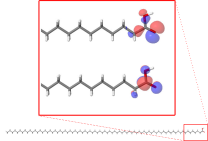
\includegraphics[scale=0.6]{Pics/NTOACID}
\caption{An interesting caption}
\end{figure}


\begin{figure}
\centering
\begin{subfigure}{0.3\linewidth}
\centering
\includegraphics[scale=0.6]{Pics/CISDENSE}
\caption{}
\end{subfigure}
$\Longrightarrow$
\begin{subfigure}{0.6\linewidth}
\centering
\includegraphics[scale=0.6]{Pics/CIS}
\caption{}
\end{subfigure}
\caption{An inte capwd m}
\end{figure}

% PAO CCLR not good! Look at Gunnar review article perhaps

% First appearance of local EOM-CCSD 
% Cra2002 https://aip.scitation.org/doi/pdf/10.1063/1.1537718

% First appearance of local CCLR CC2 (no doubles wrapping) Kat2006 https://aip.scitation.org/doi/pdf/10.1063/1.2339021
% Flaw: Domains dtermined from CCS, bad if not correponding to good approximat. ALso fixed during davidson

% Kat2009 https://aip.scitation.org/doi/pdf/10.1063/1.3237134
% FIxes Problem by refreshing domains

% state-specific PNOs from CIS(D) Hel2011 https://aip.scitation.org/doi/10.1063/1.3664902

% Hel2013 PNO-CC2 https://aip.scitation.org/doi/10.1063/1.4819071

% Hel2014 PNO-ADC2 https://www.sciencedirect.com/science/article/pii/S2210271X14001194?via%3Dihub

\section{Critical Stance on AO vs LMO} 

Distance criteria, or Mulliken/Löwdin pouplation
AO only for closed expressions (not for CCSD++) 
LOcal: ij cirteria, ij->ab criteria % https://www.sciencedirect.com/science/article/pii/S1574140006020044?via%3Dihub

\subsection{CC2}


\subsection{ADC}